\documentclass[psfig,11pt]{article} 
\usepackage{graphicx} 
\usepackage{setspace}
\textheight 24.4cm
\textwidth 16.59cm
\topmargin -0.0cm
\oddsidemargin -0.04in
\evensidemargin -0.04in

\def\normalstretch{1.0}
\def\talllinestretch{1.5}
\def\shortlinestretch{0.8}
\renewcommand{\baselinestretch}{\normalstretch}
\parskip 1ex
\renewcommand{\topfraction}{.75}
\renewcommand{\textfraction}{.20}
\renewcommand{\floatsep}{0.0pt}
\renewcommand{\textfloatsep}{1.0cm}
\renewcommand{\floatpagefraction}{.85}

\def\portindent{\hspace{\parindent}}
\newcommand{\REM}[1]{} 
\newcommand{\sol}[1]{\noindent\textcolor{red}{{#1}}}
\newcommand{\solspace}[1]{}
%\newcommand{\sol}[1]{\REM{#1}}
%\newcommand{\solspace}[1]{\vspace{#1}}

\newif\ifsol
%\soltrue


\input epsf
\usepackage{epsfig}
\usepackage{subfigure}
\usepackage{fullpage}
\usepackage{multirow}
\pagestyle{plain}
\usepackage[usenames]{color}

\begin{document}

\newcounter{quest}
\newenvironment{question}[1][??]{\noindent{\bf Question  \stepcounter{quest}
\arabic{quest} (\textrm{#1} points): }}

\begin{question}[20]
In one of your CMPUT 229 assignments you need to print the hexadecimal
representation of the 32-bit number stored in a given register. You
have already created a subroutine called {\tt PrintChar} that prints
the character represented in ASCII by the 8 least significant bits of
{\tt \$a0} to the screen. Now you have to write the subroutine that
receives as a parameter the 32-bit number whose hexadecimal
representation you want to print and prints one hexadecimal digit at a
time. Lets call this subroutine {\tt PrintHex}. To print the alpha
characters of the ASCII code, {\tt PrintHex} uses capital
letters. {\tt PrintHex} receives in {\tt \$a0} the 32-bit number to be
printed, and calls {\tt PrintChar} to print each individual
hexadecimal digit. The figure below has the ASCII code. For instance,
the ASCII code for the character {\tt R} is {\tt 0x52}. {\tt PrintHex}
must follow all the calling conventions and restrictions on operand
sizes of the MIPS architecture. (Please use the next page to write
your code and write it clearly).

\begin{center}
       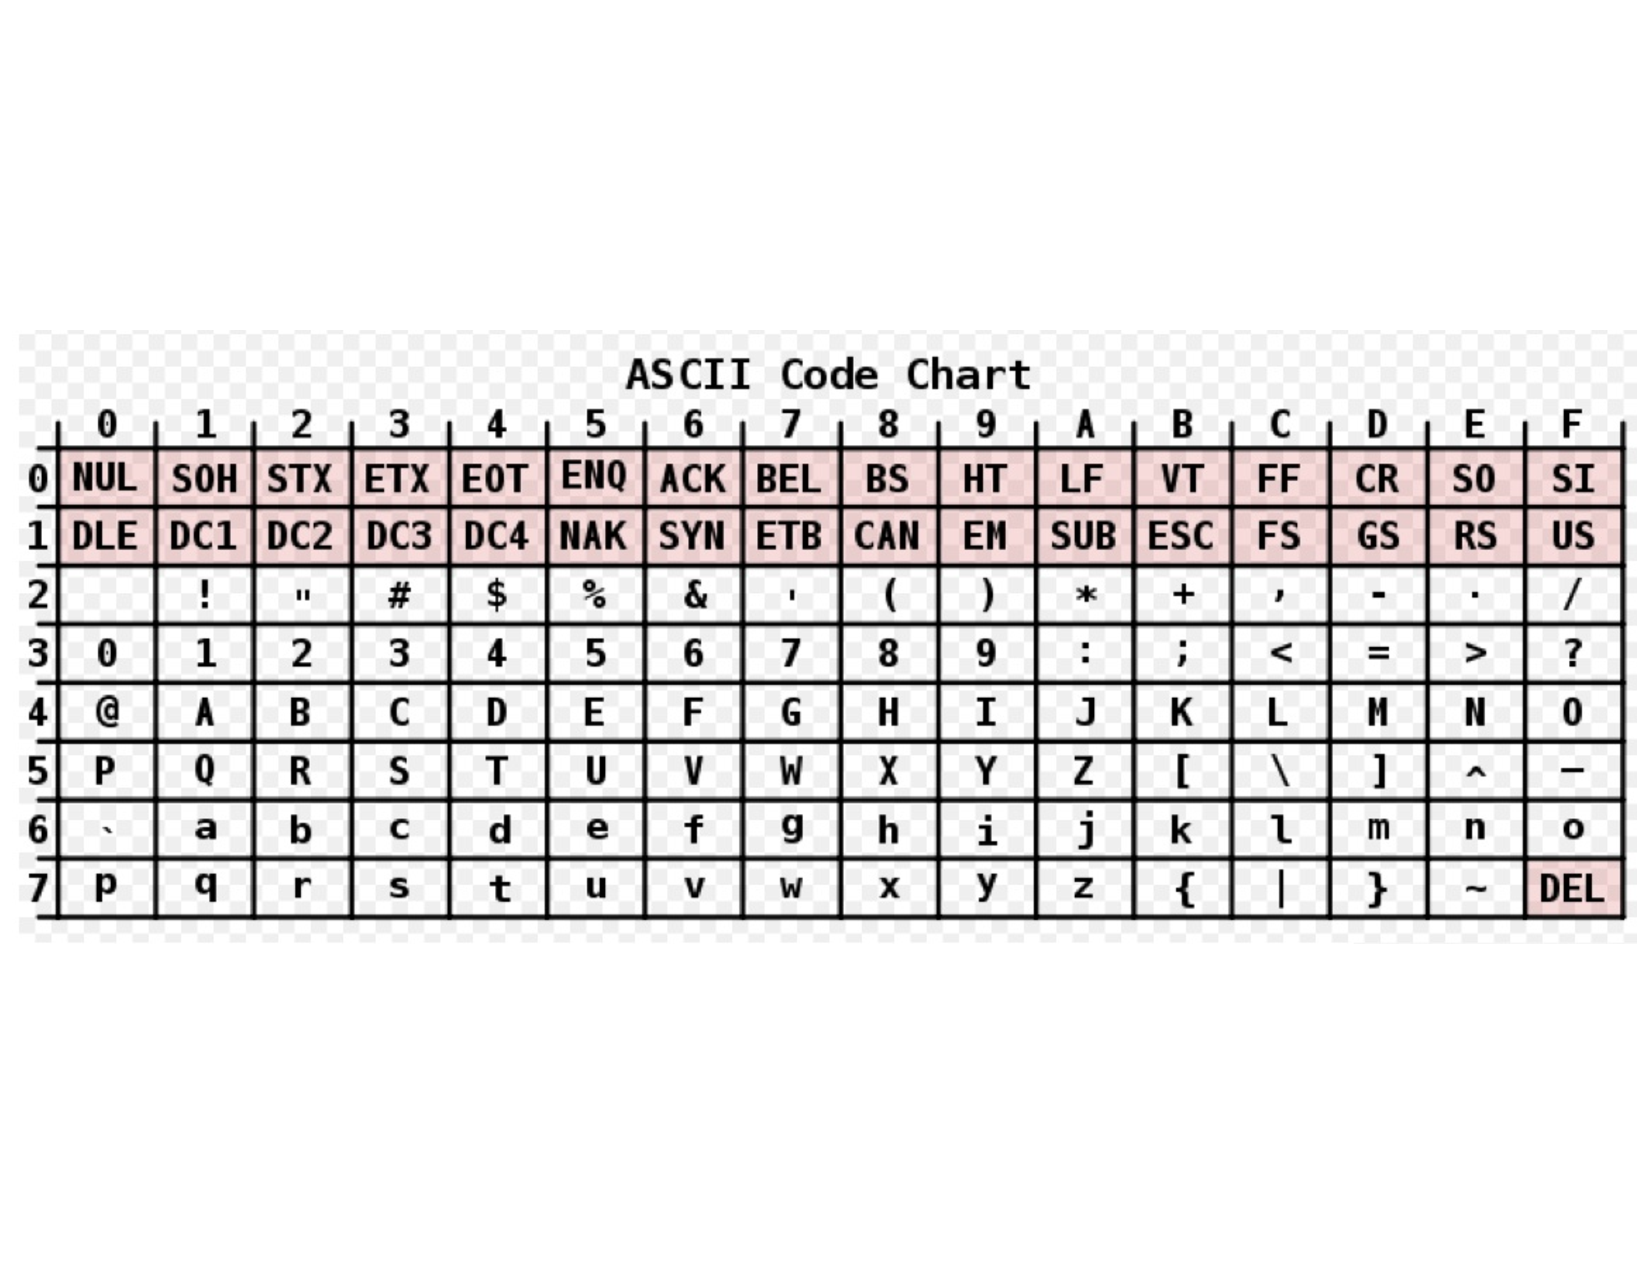
\includegraphics[width=6in]{ASCII}
\end{center}

\newpage
\ifsol
\color{red}
\begin{verbatim}
# Register usage:
#      $s0: mask
#      $s1: shfamount
#      $t2: temp
#      $t3: digit
#      $s5: number
PrintHex:
          sub  $sp, $sp,16
          sw   $ra, 0($sp)     # save $ra
          sw   $s0, 4($sp)     # save $s0
          sw   $s1, 8($sp)     # save $s1
          sw   $s5, 12(sp)     $ save $s5
          add  $s5, $a0, $zero # number <- $a0
          lui  $s0, 0xF000     # mask <- 0xF000 0000
          li   $s1, 28         # shfamount <- 28
nex_digit:
          beq  $s0, $zero, done
          and  $t2, $s5, $s0   # temp <- number & mask
          srlv $t3, $t2, $s1   # digit <- temp >> shfamount
          bgt  $t3, 9, alpha   # if digit > 9 then it is alpha
          add  $a0, $t3, 0x30  # char <- digit + 0x30
          b    print
alpha:     
          add  $a0, $t3, 0x41  # char <- digit + 0x41
print:
          jal  PrintChar
          srl  $s0, $s0, 4     # mask <- mask >> 4
          subi $s1, $s1, 4     # shfamount <- shfamount - 4
          b    next_digit
done:
          lw   $ra, 0($sp)     # restore $ra
          lw   $s0, 4($sp)     # restore $s0
          lw   $s1, 8($sp)     # restore $s1
          lw   $s5, 12(sp)     $ restore $s5
          add  $sp, $sp, 16
\end{verbatim}
\color{black}
\else
\vspace{1in}
\fi
\end{question}



\end{document}

